\documentclass[]{article}

\usepackage[T1]{fontenc}
\usepackage[utf8]{inputenc}
\usepackage[english]{babel}
\usepackage[left=1.5cm,right=1.5cm,top=2cm,bottom=2.5cm]{geometry}

\usepackage[fontsize=13pt]{scrextend}

\renewcommand{\baselinestretch}{1.3}

\usepackage[nooneline]{caption}
\usepackage{indentfirst}
\usepackage{tabularx}
\usepackage{amsmath}
\usepackage{hyperref}

\usepackage{fancyhdr}
\setlength{\headheight}{15mm}

\usepackage[pdftex]{graphicx}
\graphicspath{{img/}}

\pagestyle{fancy}
\lhead{\textbf{\normalsize Monte-Carlo Option Pricing}}
\rhead{\textbf{\normalsize Author: }\normalsize Maksim Kiryakin}


\begin{document}

{
	\Large
	\href{https://github.com/MaximKiryakin/quant-finance-projects/tree/main/monte-carlo-option-pricing}{Project repository}.
}

\section{Problem statement}

The goal of this work is to price a path-dependent derivative by Monte-Carlo simulation of the
underlying asset under the \textbf{Constant Elasticity of Variance (CEV)} model.

The CEV model generalizes geometric Brownian motion (GBM) by allowing the volatility to depend on
the price level through an elasticity parameter $\gamma$. Under the risk-neutral measure the
underlying asset $S_t$ follows

\begin{equation}
	dS_t = (r - q)\,S_t\,dt + \sigma\,S_t^{\gamma}\,dW_t,
\end{equation}

where $r$ is the risk-free rate, $q$ the continuous dividend yield, $\sigma$ the volatility scale,
$\gamma$ the elasticity of variance, and $W_t$ a standard Brownian motion. For $\gamma = 1$ the model
reduces to the Black--Scholes GBM; for $\gamma < 1$ volatility increases as the price falls,
reproducing the leverage effect observed in equity markets.

\section{Simulation scheme}

The process is discretized on a uniform grid $0 = t_0 < t_1 < \dots < t_m = T$ with step
$\Delta t = T/m$ using the Euler--Maruyama scheme:

\begin{equation}
	S_{t+1} = S_t + (r - q)\,S_t\,\Delta t + \sigma\,S_t^{\gamma}\,\sqrt{\Delta t}\,Z_t,
	\qquad Z_t \sim \mathcal{N}(0, 1),
\end{equation}

with the non-negativity constraint $S_{t+1} \leftarrow \max(S_{t+1}, 0)$ to keep simulated prices
admissible. $N$ independent paths are generated. Figure \ref{fig:paths} shows a sample of simulated
trajectories.

\begin{figure}[h!]
	\centering
	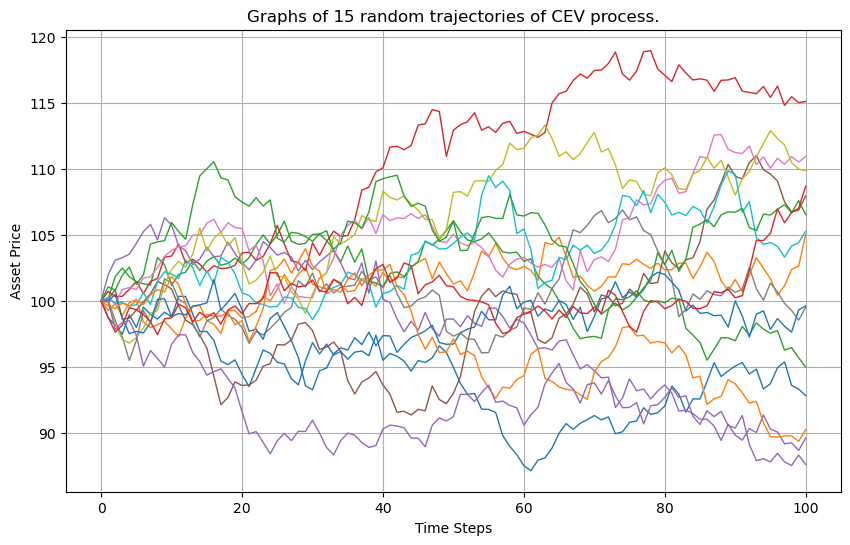
\includegraphics[width=0.85\textwidth]{cev_mc.png}
	\caption{A sample of simulated CEV price trajectories.}
	\label{fig:paths}
\end{figure}

\section{Pricing a cliquet option}

A \textbf{cliquet} (ratchet) option pays the sum of capped/floored periodic returns over a set of
reset dates. Here we consider a cliquet that pays, at each reset date $t_i = iT/n$ ($i = 1, \dots, n$),
the positive part of the price increment over the preceding period. Its discounted payoff along a
path is

\begin{equation}
	\text{Payoff} = \sum_{i=1}^{n} e^{-r t_i}\,\max\!\left(S_{t_i} - S_{t_{i-1}},\, 0\right).
\end{equation}

The Monte-Carlo price estimate and its standard error are

\begin{equation}
	\hat{P} = \frac{1}{N}\sum_{k=1}^{N} \text{Payoff}^{(k)},
	\qquad
	\widehat{\text{SE}} = \frac{\hat{\sigma}_{\text{Payoff}}}{\sqrt{N}},
\end{equation}

where $\hat{\sigma}_{\text{Payoff}}$ is the sample standard deviation of the per-path payoffs. The
standard error quantifies the Monte-Carlo sampling uncertainty and decreases as $O(N^{-1/2})$ with
the number of paths.

\section{Implementation}

The code is organized as follows:

\begin{itemize}
	\item \texttt{simulate\_cev(S0, r, q, sigma, gamma, T, m, N)} --- vectorized Euler--Maruyama
	simulation of $N$ CEV paths on an $m$-step grid.
	\item \texttt{cliquet\_price(...)} --- Monte-Carlo estimate of the cliquet price and its standard
	error from the simulated paths.
	\item \texttt{plot\_mc\_paths(...)} --- visualization of a subset of simulated trajectories.
\end{itemize}

The full experiments --- parameter choices, price estimates, and convergence of the standard error
with the number of paths --- are in the accompanying notebook \texttt{main.ipynb}.

\section{Conclusion}

The work implements Monte-Carlo pricing of a path-dependent (cliquet) option under the CEV model,
including a discretized simulation of the underlying, discounted payoff aggregation, and an estimate
of the Monte-Carlo standard error. The framework is directly extensible to other path-dependent
payoffs (Asian, barrier, lookback) by changing only the payoff function applied to the simulated paths.

\end{document}
